{\bf Problem 5: Answers}

\begin{enumerate}
    \item See Figure 8
	\begin{figure}[h!]
	    \centering
	    \caption{Linear network digit reconstructions} 
	    
\includegraphics[width=0.8\linewidth]{../figures/a5_True_actual.pdf}
	    \caption*{Actual}
	    
\includegraphics[width=0.8\linewidth]{../figures/a5_True_32.pdf}
	    \caption*{h=32 Train Error=1125.42}
	    
\includegraphics[width=0.8\linewidth]{../figures/a5_True_64.pdf}
	    \caption*{h=64 Train Error=605.77}
	    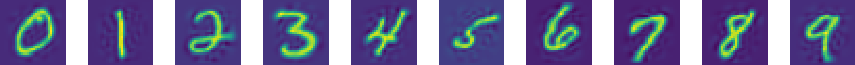
\includegraphics[width=0.8\linewidth]{../figures/a5_True_128.pdf}
	    \caption*{h=128 Train Error=280.53}	
	\end{figure}
    \item See Figure 9
	\begin{figure}[h!]
	    \centering
	    \caption{Non-linear network digit reconstructions} 
	    
\includegraphics[width=0.8\linewidth]{../figures/a5_False_actual.pdf}
	    \caption*{Actual}
	    
\includegraphics[width=0.8\linewidth]{../figures/a5_False_32.pdf}
	    \caption*{h=32 Train Error=974.97}
	    
\includegraphics[width=0.8\linewidth]{../figures/a5_False_64.pdf}
	    \caption*{h=64 Train Error=552.35}
	    
\includegraphics[width=0.8\linewidth]{../figures/a5_False_128.pdf}
	    \caption*{h=128 Train Error=316.65}
	\end{figure}
    \item 
	\hfill
	\begin{tabular}{ |c|c|c|c| }
	    \multicolumn{4}{c}{Test Errors on Linear and Non-linear networks} \\
	    \hline
	    & h=32 & h=64 & h=128 \\
	    \hline
	    Linear & 1096.89 & 590.39 & 275.92 \\
	    \hline
	    Non-linear & 958.09 & 545.69 & 315.90 \\
	    \hline
	\end{tabular}\hfill\mbox{}
    \item  See Figure 10. 
	Because of hidden layers and non-linearities, the Autoencoder is better able to capture digit features than the PCA model. 
	Compare and contrast how increasing the number of hidden layers improves the fidelity of the reconstructed digits faster than increasing k in PCA.
	Further, the Autoencoder uses activation functions for better non-linear boundaries given the non-linear model superior performance over PCA for all values of k/h.
	\begin{figure}[h!]
	    \centering
	    \caption{PCA digit reconstructions} 
	    
\includegraphics[width=0.8\linewidth]{../figures/a5_d_actual.pdf}
	    \caption*{Actual}
	    
\includegraphics[width=0.8\linewidth]{../figures/a5_d_recon_32.pdf}
	    \caption*{k=32}
	    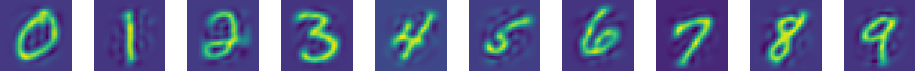
\includegraphics[width=0.8\linewidth]{../figures/a5_d_recon_64.pdf}
	    \caption*{k=64}
	    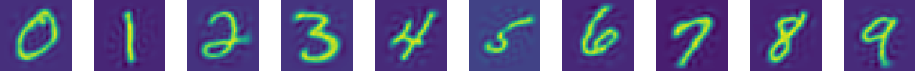
\includegraphics[width=0.8\linewidth]{../figures/a5_d_recon_128.pdf}
	    \caption*{k=128}
	\end{figure}

	
\end{enumerate}

{\bf Problem 5: Code}
\begin{quote}
    \lstinputlisting[language=Python]{../code/a5.py}
\end{quote}
